% Centralised critic network of the MAPPO coverage agent, see src/models/actor_critic.py
% (class Critic) and MultiRobotCoverageEnv.critic_inputs.
% Compile standalone:  pdflatex critic_network.tex
% Include in a paper:  \includegraphics{critic_network.pdf}
\documentclass[tikz,border=6pt]{standalone}
\usepackage[T1]{fontenc}
\usepackage{lmodern}
\usetikzlibrary{positioning,fit,backgrounds,arrows.meta,calc,shadows}

% Palette (same as policy_network.tex)
\definecolor{cIn}{HTML}{E8F1FB}    \definecolor{cInD}{HTML}{3B78C2}
\definecolor{cEnc}{HTML}{EAF7EE}   \definecolor{cEncD}{HTML}{2E8B57}
\definecolor{cMap}{HTML}{FFF4E0}   \definecolor{cMapD}{HTML}{D9822B}
\definecolor{cMem}{HTML}{F3ECFA}   \definecolor{cMemD}{HTML}{7B4FB3}
\definecolor{cOut}{HTML}{FDECEC}   \definecolor{cOutD}{HTML}{C0392B}
\definecolor{cGrey}{HTML}{6B7280}

\tikzset{
  font=\sffamily\small,
  >={Stealth[length=2.2mm]},
  block/.style={draw=#1D, fill=#1, rounded corners=3pt, line width=0.7pt,
                minimum height=8mm, minimum width=26mm, align=center,
                drop shadow={opacity=0.12, shadow xshift=0.6pt, shadow yshift=-0.6pt}},
  inp/.style={block=cIn, minimum width=30mm},
  enc/.style={block=cEnc},
  mapb/.style={block=cMap},
  memb/.style={block=cMem},
  head/.style={block=cOut},
  op/.style={circle, draw=cGrey, fill=white, line width=0.7pt, inner sep=1.2pt,
             font=\sffamily\bfseries\small},
  group/.style={draw=#1, dashed, rounded corners=6pt, line width=0.8pt, inner sep=9pt},
  title/.style={font=\sffamily\bfseries\footnotesize, text=#1},
  note/.style={font=\sffamily\scriptsize, text=cGrey, align=center},
  flow/.style={->, line width=0.8pt, draw=black!70},
}

\begin{document}
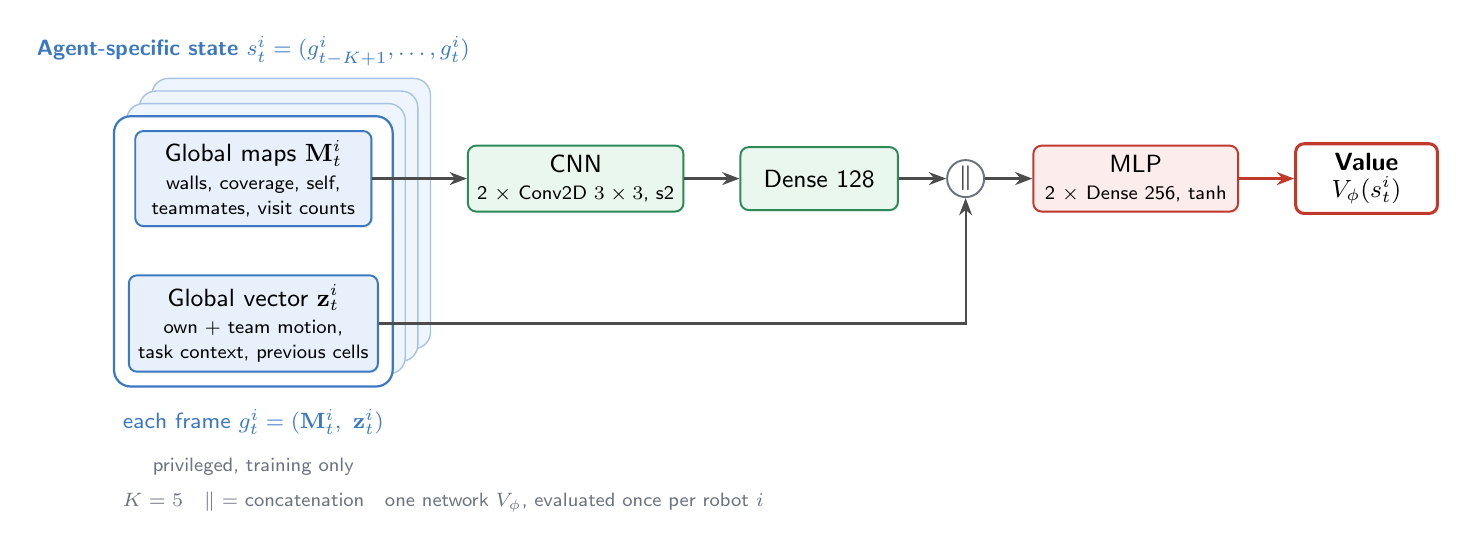
\begin{tikzpicture}[node distance=5mm and 7mm]

% ------------------------------------------------------------------ inputs
\node[inp] (gmap)
  {Global maps $\mathbf{M}_t^i$\\[-1pt]\scriptsize walls, coverage, self,\\[-2pt]\scriptsize teammates, visit counts};
\node[inp, below=6mm of gmap] (gvec)
  {Global vector $\mathbf{z}_t^i$\\[-1pt]\scriptsize own + team motion,\\[-2pt]\scriptsize task context, previous cells};

% stacked-frame look behind the two per-frame inputs
\begin{scope}[on background layer]
  \foreach \s in {3,2,1}
    \node[draw=cInD!45, fill=cIn!70, rounded corners=6pt, line width=0.5pt,
          fit=(gmap)(gvec), inner sep=5pt,
          xshift=\s*1.6mm, yshift=\s*1.6mm] {};
  \node[draw=cInD, fill=white, rounded corners=6pt, line width=0.8pt,
        fit=(gmap)(gvec), inner sep=5pt] (frames) {};
\end{scope}
\node[title=cInD, above=5mm of frames.north]
  {Agent-specific state $s_t^i = (g_{t-K+1}^i,\dots,g_t^i)$};
\node[note, below=1.5mm of frames.south, text=cInD, font=\sffamily\footnotesize] (flab) {each frame $g_t^i = (\mathbf{M}_t^i,\ \mathbf{z}_t^i)$};
\node[note, below=0.5mm of flab] {privileged, training only};

% ------------------------------------------------------------------ map encoder
\node[enc, right=12mm of gmap] (cnn) {CNN\\[-1pt]\scriptsize 2 $\times$ Conv2D $3\times3$, s2};
\node[enc, right=of cnn, minimum width=20mm] (emb) {Dense 128};
\draw[flow] (gmap) -- (cnn);
\draw[flow] (cnn) -- (emb);

% ------------------------------------------------------------------ concat + head
\node[op, right=6mm of emb] (cat) {$\Vert$};
\draw[flow] (emb) -- (cat);
\draw[flow] (gvec.east) -| (cat.south);

\node[head, right=6mm of cat] (mlp) {MLP\\[-1pt]\scriptsize 2 $\times$ Dense 256, tanh};
\node[head, fill=white, draw=cOutD, line width=1.1pt, right=of mlp, minimum width=18mm] (val)
  {\textbf{Value}\\[-1pt]$V_\phi(s_t^i)$};
\draw[flow] (cat) -- (mlp);
\draw[flow, line width=1.1pt, draw=cOutD] (mlp) -- (val);

% ------------------------------------------------------------------ legend
\node[note, align=left, anchor=north west] at ($(frames.south west)+(0,-12mm)$)
  {$K=5$\quad $\Vert$ = concatenation\quad one network $V_\phi$, evaluated once per robot $i$};

\end{tikzpicture}
\end{document}
